
\chapter{The title of chapter one}

\section{Introduction}
\label{sec:intro}

\lettrine[lines=2]{Q}{uantum effects}
effects such as entanglement and matter interference are
predicted cornerstones of future technologies. Their exploitation
requires the ability to reliably and accurately control complex
quantum systems. A major obstacle is that a quantum system
can never completely be isolated from its environment and the
interaction with the environment causes 
decoherence~\cite{BreuerBook}. This is particularly true for condensed
phase settings as encountered in, e.g., solid state quantum devices. 
A number of concepts, such as decoherence-free subspaces~\cite{LidarPRL98}
and noiseless subsystems~\cite{LorenzaSci01}, dynamical
decoupling~\cite{LorenzaPRL99} and spectral
engineering~\cite{ClausenPRL10}, have been developed to cope with 
decoherence. The applicability of these strategies is tied to specific
conditions on the interaction between system and environment and,
in practice, is often  limited to systems that can be described by simple
models. For complex quantum systems, numerical optimal control offers an
alternative approach. It calculates the external controls that
implement a desired target operation by performing an iterative search
in the parameter space of the controls~\cite{RiceBook}. 

For quantum systems that are subject to decoherence, numerical optimal
control was first employed 
to realize laser cooling of internal degrees of freedom in
molecules~\cite{BartanaJCP97}. Further applications, also utilizing a
Markovian master equation to describe the open system dynamics, 
include controlling coherences~\cite{OhtsukiJCP99}, automatic
protection against noise~\cite{KallushPRA06}, selective
photoexcitation of charge transfer~\cite{TremblayPRA08},
electric current in a molecular junction~\cite{KleinekathoeferEPJB10},
quantum gates~\cite{ToSHJPB11}, and 
quantum memories~\cite{GormanPRA12}. Due to the formal equivalence
between Markovian 
dissipation and quantum measurements, optimized observations can be
determined using the same set of tools~\cite{ShuangJCP07}. 
Numerical optimal control can also be applied to non-Markovian
quantum
systems~\cite{RebentrostPRL09,AsplundPRL11,SchmidtPRL11,FloetherNJP12} 
provided the dynamics can be calculated with sufficient efficiency. 

The question of numerical effort becomes particularly important in the
optimization of high-fidelity quantum gates. High
fidelities, or small errors,  are best achieved with monotonically convergent
optimization algorithms that utilize 
gradient information and thus require repeated forward and backward
propagation~\cite{SomloiCP93,ZhuJCP98}. Gate optimization under
coherent dynamics implies propagation of a set of states that span the 
Hilbert (sub)space on which the target is
defined~\cite{JosePRL02,JosePRA03}. For open system dynamics, this was
generalized to a set of states that span the corresponding Liouville
(sub)space~\cite{KallushPRA06,OhtsukiNJP10,ToSHJPB11,FloetherNJP12}. It
requires not only propagation of density matrices instead of
wavefunctions but also a significantly larger number of states
since Liouville space dimension is the square of Hilbert space
dimension. Realistically, this limits quantum gate optimization to but 
the simplest examples, i.e., one-qubit and two-qubit operations. 

The direct extension from Hilbert to
Liouville space~\cite{KallushPRA06,OhtsukiNJP10,ToSHJPB11} 
overlooks the fact that in quantum gate optimization,
the target is a unitary operation and not a general dynamical map. The
latter would indeed require a basis that spans the full Liouville
space. However, much less information is required to assess how
well a desired unitary is implemented. This observation is not only
relevant for optimal control but also provides the
basis for all current attempts at reducing the resources for
estimating the average gate
error~\cite{BenderskyPRL08,FlammiaPRL11,MagesanPRL11,daSilvaPRL11,ReichKochPRL13}. 
In fact, only two states are necessary to distinguish any two
unitaries, irrespective of Hilbert space
dimension~\cite{ReichKochPRA13}. 
We show here that these two states,
together with a third state enforcing the dynamical map on the
optimization subspace to be
contracting and population conserving,
can be utilized to construct an optimization functional
which attains its optimal value only if the desired gate is
implemented with unit fidelity. 

The two states that are required for unitary identification are
constructed such that the first one consists of non-degenerate
contributions from each Hilbert (sub)space direction. This corresponds
to choosing a basis, and probing the gate error within this basis. In
order to determine the error of gates that are diagonal in the chosen
basis, i.e., phase errors, the second state is needed. For Hamiltonians
which due to their inherent structure allow for nothing but diagonal gates, 
only the second state together with the third one is required, enforcing the
dynamical map on the optimization subspace to be contracting and
norm conserving. In our application, we
thus distinguish between gates which are diagonal and those that are
non-diagonal in the logical basis. 

Our optimization functional is closely related to the gate error. 
While two states represent the minimal set of states required to
distinguish any two unitaries, it is impossible to deduce bounds on
the gate error from the two
states~\cite{ReichKochPRA13}. This is due to the state corresponding to
the choice of basis being a totally mixed thermal state. Meaningful
bounds on the gate error can be derived numerically when replacing the totally
mixed state by a set of $d$ pure states where $d$ is the dimension of
Hilbert space, i.e., by choosing a separate basis state for each
Hilbert space direction~\cite{ReichKochPRA13,FiurasekPRA14}. The resulting set
consists of $d+1$ states. Analytical bounds are obtained when also the
second state of the minimal set is expanded~\cite{HofmannPRL05}. The
corresponding set is built out of the $2d$ states of two mutually
unbiased bases~\cite{ReichKochPRA13}. This observation from process
verification motivates the choice of optimization functionals which
utilize these extended sets of states. Although the
number of states then depends on Hilbert space dimension, this choice still
comes with very significant savings in the computational resources.
For example, already for a two-qubit gate,
both $2d$ and $d+1$ represent a significant reduction in the number of
states that need to be propagated, namely a reduction from 16 for the
full Liouville space basis to 8 and 5, respectively. 

We demonstrate below that two states are sufficient to
optimize diagonal gates and three states to optimize non-diagonal
two-qubit gates. We also show that, depending on the desired gate
error, $d+1$, respectively $2d$ states in the optimization functional
correspond to the numerically most efficient choice. We consider a
controlled phasegate  with neutral trapped atoms that are excited into 
a Rydberg state and a \sqrtISWAP gate with
superconducting qubits. In both examples, our optimization identifies
gate implementations for which the error is limited by
decoherence. This proves that all reduced sets of states are
sufficient for determining the fundamental limit to the gate error and
thus for quantum gate optimization. 

The paper is organized as follows. Section~\ref{sec:oct} defines 
the optimization functional and presents the optimization
algorithm. Optimization of a controlled phasegate for neutral atoms is
discussed in Sec.~\ref{sec:phasegate}, whereas optimization of a
non-diagonal gate for superconducting qubits is studied in
Sec.~\ref{sec:allgates}. Section~\ref{sec:concl}
concludes. 
The algebraic framework and the proofs required for the construction
of the three states employed in the optimization functional are
presented in Appendix~\ref{sec:proof}. 


%%%%%%%%%%%%%%%%%%%%%%%%%%%%%%%%%%%%%%%%%%%%%%%%%%%%%%%%%%%%%%%%%%%%%%%%%%%%%%%%
\section[OCT for a unitary operation under
  dissipative  evolution]{Optimal control theory for a unitary operation under
  dissipative  evolution}
\label{sec:oct}

\subsection{Optimization functional}
\label{subsec:func}
In order to employ optimal control theory to determine a
high-fidelity implementation of quantum gates, one needs to 
define a distance measure $J_T $
between the desired unitary $\Op O$ and the actual evolution. We show
here that 
\begin{equation}
  J_T = 1 - \sum_{i=1}^{n}
    \frac{w_i}{\Tr[\Op\rho_i^2(0)]} \, \mathfrak{Re}\left\{\Tr\left[
    \Op O\Op\rho_{i}(0)\Op O^{\dagger}\Op\rho_{i}\left(T\right)\right]\right\}
  \label{eq:functional}
\end{equation}
with $n=3$ and specific initial states $\Op\rho_i(0)$ represents
a suitable choice for $J_T$. This is in contrast to
Refs.~\cite{KallushPRA06,OhtsukiNJP10,ToSHJPB11}, where $n$ was taken
to be the Liouville space dimension corresponding to $\Op O$, 
i.e., $n=2^{2N}$ for $N$ qubits,
and $\Op\rho_i$ an orthonormal basis (under the Hilbert-Schmidt
product) of Liouville space.
In Eq.~\eqref{eq:functional}, $w_i$ are  weights,
normalized as $\sum_{i=1}^n w_i = 1$. In order to evaluate $J_T$, 
the time evolved states $\Op\rho_i(T)$
need to be obtained by solving the equation of motion describing the open
system's evolution for $\Op\rho_i$. While in general the dynamics can
be non-Markovian, we will restrict ourselves to a Markovian master
equation in the examples below. We assume the coherent part to include
coupling to 
an external control, i.e., the Hamiltonian is of the form $\Op
H(t)=\Op H_0 + \epsilon(t)\Op H_1$, and generalization to several
controls $\epsilon_i(t)$ is straightforward.

The functional $J_T$ needs to be minimized
with respect to $\epsilon(t)$.
Further constraints can be added, for example,
\begin{equation}
  \label{eq:J}
  J = J_T -
  \lambda_a\int_0^T\left[\epsilon(t)-\epsilon_{\text{ref}}(t)\right]^2/S(t) \dd t\,,
\end{equation}
where $\epsilon_{\text{ref}}(t)$ denotes a reference field, $S(t)$ enforces
the field to be smoothly switched on and off,
and the second term in Eq.~\eqref{eq:J} ensures a finite pulse
fluence~\cite{JosePRA03}. More complex additional constraints, for
example restricting the spectral width of the pulse or confining the
accessible state space~\cite{ReichKochJMO13,JosePRA13}, are also
conceivable. 
 
Mathematically, our claim  that only three states are sufficient to
determine proper implementation of the desired unitary $\Op O$ 
is equivalent to the conjecture that the optimization functional
attains its global minimum if and only if
\begin{equation}
  \label{eq:cond}
  \Op\rho_{i}\left(T\right) =
  \Op O\Op\rho_{i}(0)\Op O^{\dagger}
\end{equation}
for the three states $\Op\rho_i$. The three states are constructed
such that the first one fixes a basis, and the corresponding
Hilbert-Schmidt product in Eq.~\eqref{eq:functional} checks whether
the gate is correctly implemented in this basis. It misses errors
for gates that are diagonal in the basis, i.e., phase
errors~\cite{ReichKochPRA13}. The second state is therefore chosen to
detect phase errors with its Hilbert-Schmidt product in
Eq.~\eqref{eq:functional}~\cite{ReichKochPRA13}. The Hilbert-Schmidt
product of the third state determines 
whether the dynamical map attained at time $T$ conserves the
population within the optimization subspace. This is necessary since
the time evolution can  be non-unitary due to decoherence or due to
leakage into states other than the logical basis~\footnote{%
  Strictly speaking, one should enforce the dynamical map on the
  optimization subspace to be unital, i.e., both norm conserving
  and contracting. This could only be achieved by employing the trace
  distance  of the ideal and actually time evolved third state,
  not their Hilbert Schmidt product, in the optimization functional,
  cf. Appendix~\ref{sec:proof}. However, for all practical purposes,
  the Hilbert Schmidt product turns out to be sufficient.
}. 

In more technical terms, $\Op\rho_{1}(0)$ is a density matrix with $N$
non-degenerate,  non-zero eigenvalues.
Spanning the $d$-dimensional Hilbert space ($d=2^N$ for $N$ qubits)
by an arbitrary complete
orthonormal basis, $\{|\varphi_i\rangle\}$,
$\Op\rho_{1}(0)$ is expressed in terms of a complete
set of $d$ one-dimensional orthogonal projectors
$\Op P_i=|\varphi_i\rangle\langle\varphi_i|$, i.e., 
$\Op\rho_{1}(0) = \sum_{i=1}^d\lambda_i \Op P_i$ with
$\lambda_i\neq\lambda_j\forall i\neq j$ and $\lambda_i\ge
0$~\cite{ReichKochPRA13}. The  
second state, $\Op\rho_{2}(0)$, is constructed to be
totally rotated with respect to $\Op\rho_{1}(0)$, i.e.,
$\Op\rho_{2}(0)=\Op P_{TR}$ where $\Op P_{TR}$ is a
one-dimensional projector obeying $\Op P_{TR}\Op P_i\neq 0$ for
$i=1,\ldots,d$~\cite{ReichKochPRA13}.
$\Op\rho_{3}(0)$ is the identity in the optimization subspace. A
possible choice for the initial states reads
\begin{subequations}\label{eq:rhos}
  \begin{eqnarray}
    \left(\Op\rho_{1}(0)\right)_{ij} & = &
    \frac{2\left(d-i+1\right)}{d\left(d+1\right)}\delta_{ij}\,,\label{eq:rho1}\\
    \left(\Op\rho_{2}(0)\right)_{ij} &=& \frac{1}{d}\,,\label{eq:rho2}\\
    \left(\Op\rho_{3}(0)\right)_{ij} &=& \frac{1}{d}\delta_{ij}\,,\label{eq:rho3}    
  \end{eqnarray}
\end{subequations}
where the matrix elements are given in the optimization subspace,
all other elements are zero.
We show in Appendix~\ref{sec:proof} that the optimization reaches its target
if and only if condition~\eqref{eq:cond} is fulfilled. Specifically, we
prove that propagation of three states is sufficient, irrespective of
the dimension of the optimization subspace. Already for a small number
of qubits, this represents a
significant computational saving compared to the propagation of $2^{2N}$
initial states deemed necessary in the
literature~\cite{KallushPRA06,OhtsukiNJP10,ToSHJPB11}.

The states $\Op\rho_1$ and $\Op\rho_2$ of Eq.~\eqref{eq:rhos}, while
sufficient in principle to distinguish any two unitaries, do not allow
for stating bounds on the gate
error~\cite{ReichKochPRA13}. Meangingful bounds on the gate error can
be obtained numerically by replacing $\Op\rho_1$, 
$\Op\rho_2$ by a set of $d+1$ states, whereas analytical
bounds can be deduced from  $2d$
states~\cite{ReichKochPRA13,HofmannPRL05,FiurasekPRA14}. Motivated by this fact, 
we define two additional sets of states that can be employed in
Eq.~\eqref{eq:functional}. When $n$ in Eq.~\eqref{eq:functional} is
taken to be  equal to $d+1$, the totally mixed state of
Eq.~\eqref{eq:rho1} is replaced by $d$ pure states, 
\begin{equation}
  \label{eq:rho1_dp1}
  \Op\rho_j(0) = |\varphi_j\rangle\langle\varphi_j|\,,
\end{equation}
with $j=1,\ldots,d$ and $\{|\varphi_j\rangle\}$ the logical basis. 
$\Op\rho_{d+1}(0)$ is simply equal to $\Op\rho_2(0)$ of
Eq.~\eqref{eq:rho2}. In this case, Eq.~\eqref{eq:rho3} is not required since
the $d+1$ pure states are sufficient to enforce the dynamical map on
the optimization subspace to be contracting and norm conserving.
Similarly, the functional~\eqref{eq:functional} employing
$n=2d$ states is constructed by replacing $\Op\rho_1(0)$ of
Eq.~\eqref{eq:rho1} by $\Op\rho_j$, $j=1,\ldots,d$ of 
Eq.~\eqref{eq:rho1_dp1} and $\Op\rho_2(0)$ of
Eq.~\eqref{eq:rho2} by
\begin{equation}
  \label{eq:rho2_2d}
  \Op\rho_{d+j}(0) = |\tilde\varphi_{j}\rangle\langle\tilde\varphi_{j}|\,,
\end{equation}
with $j = 1,\dots,d$,
where the states $\Ket{\tilde\varphi_j}$ form a mutually unbiased basis with
respect to the canonical basis $\{\Ket{\varphi_j}\}$. For two
qubits  ($d=4$), an example for such a basis is given by 
\begin{subequations}\label{eq:mub}
  \begin{eqnarray}
    \Ket{\tilde\varphi_{1}}
    &=& \frac{1}{2} \left( \Ket{00} + \Ket{01} + \Ket{10} + \Ket{11} \right) \,,\\
    \Ket{\tilde\varphi_{2}}
    &=& \frac{1}{2} \left( \Ket{00} - \Ket{01} + \Ket{10} - \Ket{11} \right) \,,\\
    \Ket{\tilde\varphi_{3}}
    &=& \frac{1}{2} \left( \Ket{00} + \Ket{01} - \Ket{10} - \Ket{11} \right) \,,\\
    \Ket{\tilde\varphi_{4}}
    &=& \frac{1}{2} \left( \Ket{00} - \Ket{01} - \Ket{10} + \Ket{11} \right) \,.
  \end{eqnarray}
\end{subequations}


\subsection{Optimization algorithm}
\label{subsec:krotov}

We assume in the following a coupling to the external field that is linear
in the field and equations of motion that are linear in the
states~\footnote{%
  A generalization to non-linear couplings and equations of motion is
  straightforward following Ref.~\cite{ReichKochJCP12}.}.
Moreover, the full optimization functional,
Eq.~\eqref{eq:J}, is linear in the states $\Op\rho_i(T)$ and does
not depend on the states at intermediate times $t$. In this case, the 
linear version of Krotov's method is sufficient to yield a
monotonically convergent optimization
algorithm~\cite{ReichKochJCP12}. It is given in terms of coupled
control equations that need to be solved simultaneously.
Here, we model the dissipative time evolution by a
Markovian master equation,
\begin{equation}
  \label{eq:LvN}
  \frac{d\Op\rho}{dt} = \mathcal{L}(\Op\rho) = -i[\Op H(t),\Op\rho]
  +\mathcal{L}_D(\Op\rho)\,.
\end{equation}
The control equations then read
\begin{subequations}\label{eq:control}
  \begin{eqnarray}
    \label{eq:forward}
    \frac{d\Op\rho_i}{dt} &=& -i[\Op H,\Op\rho_i] +\mathcal{L}_D(\Op\rho_i)\,,\\    
    \label{eq:backward}
    \frac{d\Op\sigma_i}{dt}
    &=& -i[\Op H,\Op\sigma_i] -\mathcal{L}_D(\Op\sigma_i)
    % \,,\\  \label{eq:T}
    \quad\mathrm{and}\quad
    \Op\sigma_i(t=T) =
    \frac{w_i}{\Tr[\Op\rho_i^2(0)]}
     \Op O \Op \rho_i(0) \Op O^{\dagger}\,,\\
     \label{eq:update}
     \Delta\epsilon(t) &=&
     \frac{S(t)}{\lambda_a} \sum_{i=1}^n \Im\left\{
     \Tr\left(
       \Op\sigma_i^{\old}(t)
       \frac{\partial \mathcal{L}\left(\Op\rho_i\right)}{\partial \epsilon}
       \Big|_{\rho_i^\mathrm{new},\epsilon^\mathrm{new}}
     \right)\right\}
   \end{eqnarray}
\end{subequations}
with $i=1,2,3$ when the initial conditions $\Op\rho_i(0)$
of Eq.~\eqref{eq:rhos} are
employed or $i=1,\ldots d^2$ with $d$ the dimension of Hilbert space
when a full basis of Liouville space is propagated.
In Eq.~\eqref{eq:update},
the states $\Op\sigma^{\old}_i$ are backward-propagated with the 
pulse of the previous iteration ('old'), whereas the states
$\Op\rho^{\new}_i$ are forward-propagated with the updated 
pulse ('new'). The derivative with respect to the field is given by
the commutator
\begin{equation}
\frac{\partial \mathcal{L}\left(\Op\rho\right)}{\partial \epsilon}
= -i \left[\frac{\partial \Op H}{\partial \epsilon}, \Op{\rho} \right]
\end{equation}
and has to be evaluated for the `new' field and the states $\Op\rho$ propagated
under the `new' field. For a complex control, which
occurs for example when using the rotating wave approximation (RWA),
Eq.~\eqref{eq:update} holds for both the real and the imaginary part
of   $\epsilon(t)$. 

The value of the optimization functional in Eq.~(\ref{eq:functional}) depends on
the number and the specific choice of initial states as well as the choice of
weights. It is therefore not suitable to compare the convergence behavior
between different sets of states. Instead, we employ the average gate
fidelity, 
\begin{equation}
  F_{\avg} = \int \langle \Psi | \Op{O}^{\dagger}
              \mathcal{D}(\Ket{\Psi}\!\Bra{\Psi}) 
             \Op{O} | \Psi \rangle \dd \Psi\,,
  \label{eq:Favg}
\end{equation}
for the comparison. 
In Eq.~\eqref{eq:Favg}, $\mathcal D$ denotes the dynamical map
describing the time evolution of the open quantum system, i.e.,
$\Op\rho(T)=\mathcal D\left(\Op\rho(0)\right)$.
The gate fidelity, respectively the gate error, $1 - F_{\avg}$, is easily
evaluated as~\cite{PedersenPLA07} 
\begin{equation}
  F_{\avg} = \frac{1}{d (d+1)} \sum_{i,j=1}^d \left(
              \langle \varphi_i |
                \Op{O}^\dagger
                \mathcal{D}(\Ket{\varphi_i}\!\Bra{\varphi_j}) 
                \Op{O} |
              \varphi_j \rangle
              + \Tr\left[
                \Op{O}\Ket{\varphi_i}\!\Bra{\varphi_i}\Op{O}^{\dagger}
                \mathcal{D}(\Ket{\varphi_j}\!\Bra{\varphi_j}) 
              \right]
           \right)\,.
\end{equation}

\section{Example I: Diagonal gates}
\label{sec:phasegate}

\begin{figure}[tb] % FIG 01
  \centering
  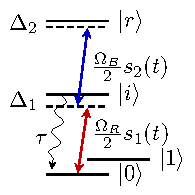
\includegraphics{figures/1q_levels}
  \caption{Atomic levels for two-photon near-resonant excitation to a
    Rydberg state.} 
  \label{fig:levels}
\end{figure}
It is quite common that a two-qubit 
Hamiltonian allows only for diagonal gates, such as a controlled
phasegate. A prominent example are non-interacting
qubit carriers that interact only when excited into an auxiliary state
where they accumulate a non-local phase~\cite{JakschPRL00}.
Neutral trapped atoms with long-range interaction in a Rydberg
state present a physical implementation of this
setting~\cite{JakschPRL00,SaffmanRMP10}.
Optimal control theory has been employed before to determine the
minimum time in which a controlled phasegate can be
implemented~\cite{GoerzKochJPB11} and the optimum distribution of the
single-qubit phases~\cite{MuellerKochPRA11}. These optimizations were
carried out, however, without explicitly accounting for decoherence.
It is thus not clear whether the best solutions to avoid decoherence
have indeed been identified. 
While the logical basis states and the Rydberg state are typically
very long-lived, the main source of decoherence is spontaneous decay
from an intermediate state which is necessary to access the Rydberg
state. 
Due to experimental feasibility, the excitation to the Rydberg state
proceeds by a near-resonant two-photon process.
The corresponding single atom Hamiltonian in the basis
$\{\Ket{0},\Ket{1},\Ket{i},\Ket{r}\}$, cf. Fig.~\ref{fig:levels}, and 
employing a two-color rotating wave approximation is given by
\begin{subequations}
  \label{eq:H_Ryd}
\begin{equation}
  \label{eq:H_1atom}
  \Op{H}_{1q} =
  \begin{pmatrix}
    0  & 0  & \frac{1}{2}\Omega_R(t) & 0                    \\
    0  & E_1 & 0                         & 0                    \\
    \frac{1}{2} \Omega_R(t)  & 0  & \Delta_1 & \frac{1}{2}\Omega_B(t)  \\
       0  & 0  & \frac{1}{2} \Omega_B(t) & \Delta_2
     \end{pmatrix}\,.
\end{equation}
The total Hamiltonian for two atoms includes an 
interaction when both atoms are in the Rydberg state, 
\begin{equation}
  \label{eq:H_2atom}
  \Op H = \Op H_1\otimes\openone + \openone\otimes\Op H_1
  - U |rr\rangle\langle rr|\,.
\end{equation}
\end{subequations}
Spontaneous emission from the intermediate level is accounted for by
the dissipator 
\begin{equation}
  \label{eq:L_atom}
  \mathcal L_D(\Op\rho) = \gamma \left(
    \Op{A} \Op{\rho} \Op{A}^\dagger
    - \frac{1}{2} \left\{\Op{A}^\dagger \Op{A}, \Op{\rho} \right\}
  \right) \quad\mathrm{with}\quad
    \Op{A} = \Ket{0}\Bra{i}\,,
\end{equation}
and $\gamma$ the decay rate, $\gamma=1/\tau$. 
The parameters correspond to optically trapped rubidium atoms 
and are summarized in Table~\ref{tab:atom}.
Since qubit level $|1\rangle$ remains decoupled throughout the
time evolution, cf. Eq.~\eqref{eq:H_1atom} and Fig.~\ref{fig:levels},
the Hamiltonian~\eqref{eq:H_Ryd} admits only diagonal gates.
\begin{table}[tb]
  \centering
 \begin{tabular}{|l|r|}\hline
  single-photon detuning $\Delta_1$                 & 600~MHz \\ \hline
  two-photon detuning $\Delta_2$                 & 0 \\ \hline
  excitation energy  $E_1$                      & 6.8~GHz \\ \hline
  Rabi frequencies  $\Omega_R$, $\Omega_B$      & 300~MHz \\ \hline
  interaction energy  $U$                        & 50~MHz \\ \hline
  lifetime $\tau = 1/\gamma$ & 25~ns \\\hline
 \end{tabular}
  \caption{Parameters of the Hamiltonian, Eq.~\eqref{eq:H_Ryd},
    for implementing a controlled phasegate with two rubidium
    atoms.}
  \label{tab:atom}
\end{table}
The update equations for real and imaginary part of the red and blue
pulses are obtained by evaluating Eq.~(\ref{eq:update}) for the
Hamiltonian given in Eq.~(\ref{eq:H_Ryd}), 
\begin{subequations}\label{eq:control_Ryd}
\begin{eqnarray}
  \label{eq:Re}
  \Re\left\{\Delta \Omega_{R,B}(t)\right\}
  & = &\frac{S(t)}{\lambda_a}
   \sum_{i=1}^{n} \Im\left\{\Tr \left(
      -i \Op\sigma_{i}^{\old}(t)
      \, \left[\Op\mu_{R,B}(t),
        \Op\rho_{i}^{\new}(t) \right]
    \right)\right\}\\ \label{eq:Im}
  \Im\left\{\Delta \Omega_{R,B}(t)\right\}
  & =& \frac{S(t)}{\lambda_a}
  \sum_{i=1}^{n}   \Im\left\{\Tr \left(
      \Op\sigma_{i}^{\old}(t)
      \, \left[\Im\left\{\Op\Omega_{R,B}(t)\right\},
        \Op\rho_{i}^{\new}(t)\right]
    \right)\right\}\,,
\end{eqnarray}  
\end{subequations}
where $\Op{\Omega}_{R,B}$ represents the 
coupling to the red and blue laser,
respectively, in Eq.~(\ref{eq:H_Ryd}). 

\begin{figure}[tb] % FIG 02
  \centering
 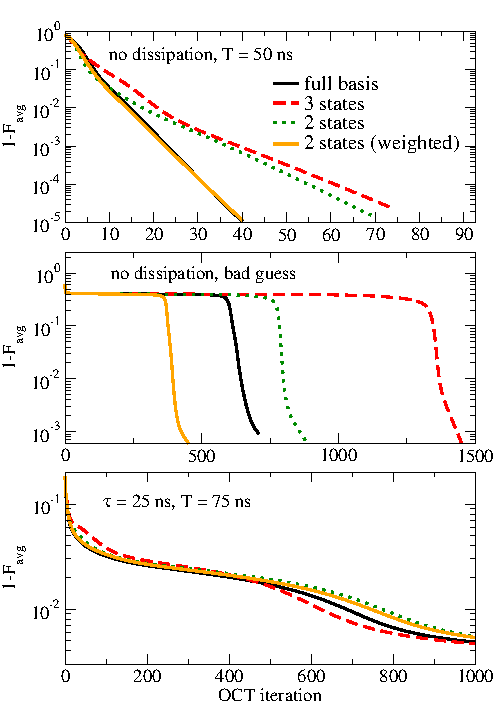
\includegraphics{figures/f_avg_combined}
 \caption[Optimizing a controlled phasegate for two trapped neutral
   atoms that are excited to a Rydberg state.]{Optimizing a controlled phasegate for two trapped neutral
   atoms that are excited to a Rydberg state. The convergence is shown
   as the gate error $1-F_{\avg}$ over OCT iterations, using  the full basis of
   16 states, as well as a reduced set of three and two propagated states,
   indicated by the same line style and colors in all panels.  The
   calculations employ equal weights of all states, except for those shown in
   orange where $w_2 / w_3 = 10$.  The top panel shows the optimization without
   any dissipation; the middle panel shows the same optimization as the top
   panel, but starting from a badly chosen guess pulse; and the bottom panel
   takes into account spontaneous emission from the intermediary state, with
   a lifetime of $\tau = 25$~ns. The gate duration is $T=50$~ns for the top and
   middle panel, and $T=75$~ns for the bottom panel. The number of iterations
   and the reached gate fidelity differ significantly in all three situations,
   hence the different ranges both for the x-axes and the y-axes.}
  \label{fig:converg:Rydberg}
\end{figure}


